\section{System Model}
%----------------------------------------------------------------------------------------%
\subsection{Network Model}
We consider an edge computing system with $K$ Access Points (APs) and $M$ edge servers, which are connected in a network as illustrated in Fig.\ref{fig:system}.
The sets of APs and edge servers are denoted as $\apSet \define \set{1,\dots,K}$ and $\esSet \define \set{1,\dots,M}$, respectively.
Each AP collects the computation jobs from the mobile users within its coverage, and makes decision on the processing edge servers from the set $\esSet$.
\comment{
    Due to the limitation of network topology, each AP could only dispatch the computation jobs to a subset of edge servers, which is denoted as \emph{candidate set} $\esSet_{k} \subseteq \esSet$ ($\forall k\in\apSet$).
}

In this paper, we shall focus on the decentralized dispatcher design at each AP.
Specifically, each AP and edge server periodically broadcast their state information (e.g., edge server dispatching choice for each job type, list of jobs being uploaded from APs to edge servers, computing queue length and etc.).
One AP updates its strategy on job dispatching when receiving the \comment{partial broadcast state information which is enough its decision making}.
Due to random transmission latency in the network, it is not sure when one AP can receive the \comment{complete partial broadcast information}, and the dispatching design could take this practical issue into consideration.

\begin{figure}[ht]
    \centering
    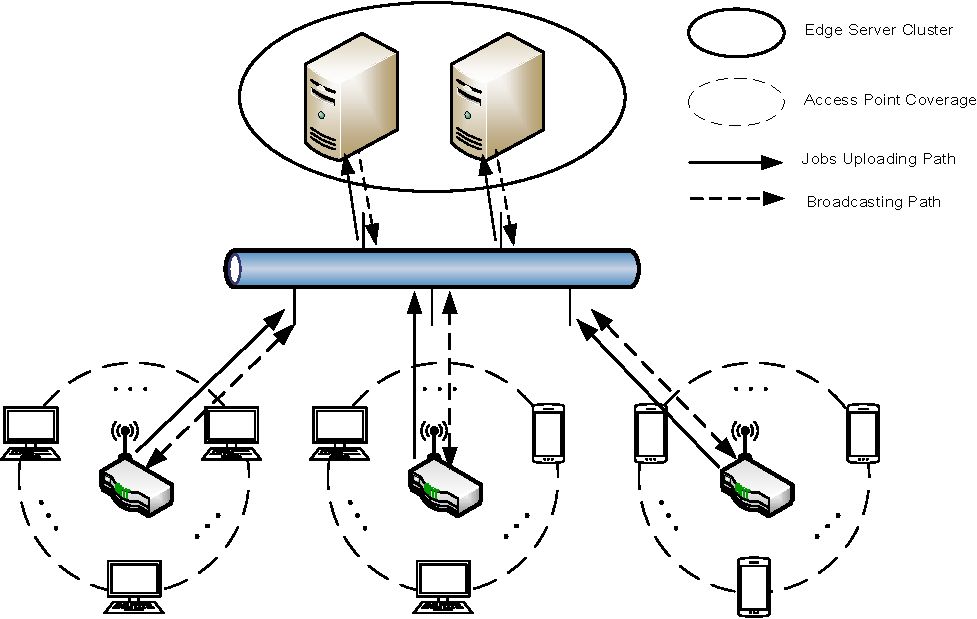
\includegraphics[width=0.80\textwidth]{system-model.pdf}
    \caption{The Illustration of MEC System Model}
    \label{fig:system}
\end{figure}

%NOTE: [job space support and arrival process]
Without loss of generality, it is assumed that there are $J$ types of computation jobs supported in this system, which are denoted via the set $\jSpace \define \set{1,\dots,J}$.
The time axis of each AP is organized by time slots.
The job arrivals in each time slot are modelled via independent Bernoulli distributions.
Specifically, the arrivals of the $j$-th job type at the $k$-th AP in different time slots are independent and identically distributed (i.i.d.) Bernoulli random variables, and the arrival probability is denoted as $\lambda_{k,j}$ ($\forall k\in\apSet, j\in\jSpace$).

%NOTE: [uploading process]
Each AP then immediately dispatches each type of received jobs to one edge server.
Let \comment{$\omega_{k,j} \in \esSet_{k}$} denotes the index of edge server for the processing of the $j$-th types of jobs dispatched from the $k$-th AP ($\forall k\in\apSet, j\in\jSpace$).
Different types of jobs may have different distributions on the input data size.
Moreover, due to the random traffic in the network, the job uploading from one AP to one edge server consumes a random number of time slots.
It's assumed that the distributions of uploading delays are independent between any two uploading jobs.
Hence, we denote $\mathcal{U}_{k,m,j}$ as the uploading delay distribution ranged in $(0, \Xi]$ (with the unit of time slot) for the $j$-th type of jobs from the $k$-th AP to the $m$-th edge server with support ($\forall k\in\apSet, m\in\esSet_{k}, j\in\jSpace$).
In practice, the distribution of uploading delay may not be known to the APs or edge servers in advance.
\delete{v4}{
    It's assumed that the distributions of uploading delays are independent between any two uploading jobs.
    Denote the uploading delays are i.i.d for the $j$-th type of jobs from the $k$-th AP to the $m$-th edge server, which is denoted as $\mathcal{U}_{k,m,j}$ ranged in $(0,\Xi]$ with the unit of time slot ($\forall k\in\apSet, m\in\esSet, j\in\jSpace$).
}

%NOTE: [processing process]
There are $J$ virtual machines (VMs) on each edge server for the computation of $J$ job types, respectively.
Different edge servers have different processing capability on different job types.
For each type, the uploaded jobs are computed in a First-Come-First-Serve (FCFS) manner.
Hence, a processing queue with maximum $L_{max}$ jobs is established for each VM.
The arrival jobs will be discarded when the processing queue is full.
Furthermore, we adopt the \emph{unrelated machines} assumption in \cite{tan-online} for job processing on edge servers.
Specifically, it is assumed that different types of jobs on different edge servers have different distributions of computing time.
\comment{
    The computing processing is formulated as memory-less Geometric process, and we denote $C_{m,j}$ as the computing time distribution (with the unit of time slot) of the $j$-th job type on the $m$-th edge server.
    The probability mass function (PMF) of $C_{m,j}$ is denoted as $f_{m,j}(k) \define (1-\frac{1}{c_{m,j}})^{k-1} \frac{1}{c_{m,j}}$ with expectation $c_{m,j}$.
}

\delete{v5}{
    The job processing time on different servers are random and machine dependent, which implies that different types of jobs on different edge servers have different processing time distributions.
    We denote $\mathcal{C}_{m,j}$ as the processing time distribution of the $j$-th type job on the $m$-th edge serer, whose range is in $(0, c_{m,j}]$ with the unit of time slot ($\forall m\in\esSet, j\in\jSpace$).
}

%----------------------------------------------------------------------------------------%

\subsection{Periodic Broadcast of State Information}
%NOTE: Periodic Broadcast is Indispensable
In our system, each AP dispatches different types of computation jobs in a fully cooperative manner, where the jobs are dispatched to achieve a global optimality.
To facilitate such dispatching decision, each AP should collect the information from other APs and edge servers.
It's assumed that every APs and edge servers broadcast their information every $t_B$ time slots as depicted in Fig.\ref{fig:brd-timeline}.
\delete{v4}{
    Furthermore, we denote $({t,n})$ as the $n$-th time slot in $t$-th broadcast interval, which is the interval between $(t-1)$-th and $t$-th broadcast ($t\in\domP$).
    Especially, we have $({t}) \define ({t,0})$ as the index of $t$-th broadcast time slot and call it $t$-th \brpoint~($t\in\domP$).
}
\begin{figure}[ht]
    \centering
    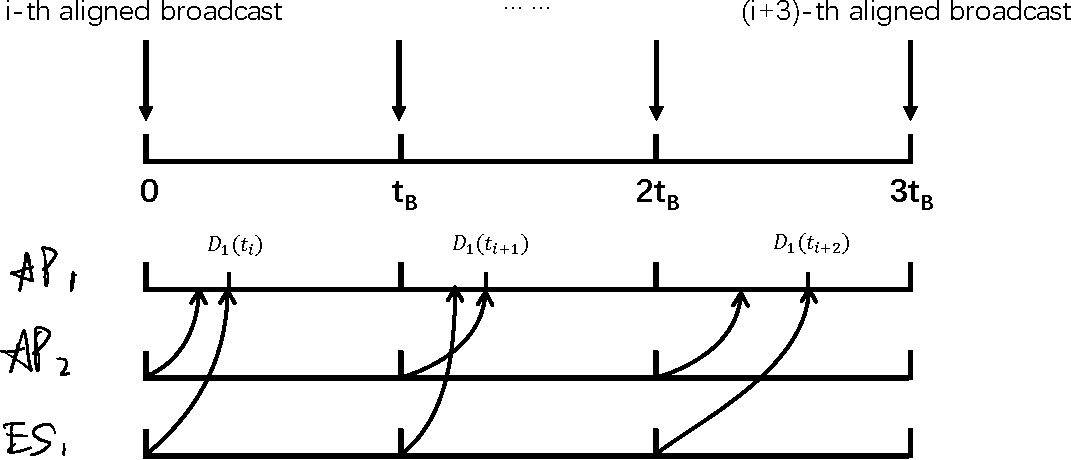
\includegraphics[width=0.80\textwidth]{brd-timeline.pdf}
    \caption{The Timeline Illustration of State Information Broadcast and Receiving}
    \label{fig:brd-timeline}
\end{figure}

%NOTE: State and Broadcast Information for AP
One AP shall maintain information about the number of jobs still in uploading. 
And due to the uploading time of one job is unknown until it's been uploaded, it further has counters to record the elapsed time slots for each job.
More specifically, at the $n$ time slot in the $t$-th interval, the number of the $j$-th type job been uploaded to the $m$-th edge server $\xi$ time slots ago from $k$-th AP is denoted as $R^{(k)}_{m,j,\xi}({t,n})$ ($\forall k\in\apSet, m\in\esSet, j\in\jSpace, \xi\in(0,\Xi]$).
The broadcast information of the $k$-th AP at the $t$-th broadcast ($t\in\domZ$) includes the information about uploading job and the dispatching decision for each type of jobs, which is defined as follows.
\comment{
    \begin{align}
        \mathcal{R}_{k}({t}) \define \set{\vec{R}^{(k)}_{m,j}({t}), \set{\omega_{k,j}(t)|\forall j\in\jSpace} | \forall m\in\esSet, j\in\jSpace},
    \end{align}
}
where $\vec{R}^{(k)}_{m,j} \define ( R^{(k)}_{m,j,0},\dots,R^{(k)}_{m,j,\Xi} )$ denotes the vector of random variables for convenience.

%NOTE: State and Broadcast Information for ES
One edge server shall maintain information about the computing queue status for each VM.
\comment{
    More specifically, at the $n$ time slot in the $t$-th interval, the $m$-th edge server have $Q_{m,j}({t,n})$ denote the pending number of the $j$-th type job ($\forall m\in\esSet, j\in\jSpace$).
    The broadcast information of the $m$-th edge server at the $t$-th ($t\in\domZ$) broadcast is defined as follows.
    \begin{align}
        \mathcal{Q}_{m}({t}) \define \set{Q_{m,j}({t}) | \forall j\in\jSpace}.
    \end{align}
    And the whole broadcast information from all APs and edge servers at the $i$-th broadcast ($i\in\domZ$) is denoted as:
    \begin{align}
        \Obsv^{\dagger}(t) \define
            \Brace{
                \mathcal{R}_{k}({t}), \mathcal{Q}_{m}({t}) | \forall k\in\apSet, m\in\esSet
            },
    \end{align}
}

%NOTE: Conflict of AP set and partial information definition
\begin{figure}[ht]
    \centering
    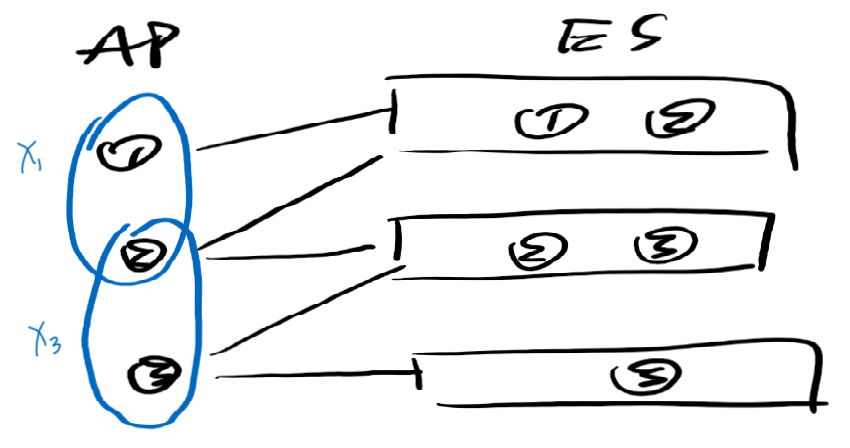
\includegraphics[width=0.80\textwidth]{images/draft-conflict.png}
    \caption{The Example Illustraction of Conflict Set and Partial Broadcast Information}
    \label{fig:conflict}
\end{figure}

According to Fig.\ref{fig:brd-timeline}, different APs would receive different parts of broadcast information at different time slots.
\comment{
    Specifically, each AP would require only partial braodcast information to help it make dispatching decision.
    We denote the \emph{conflict set} for the $k$-th AP ($\forall k\in\apSet$) as follows.
    \begin{align}
        \mathcal{X}_k \define \set{\forall k' \neq k\in\apSet|\esSet_{k'} \cap \esSet_{k} \neq \emptyset}
    \end{align}
    The \emph{conflict set} indicates the subset of APs whose status information could affect the decision making for the $k$-th AP.

    Hence, each AP would only require the broadcast information from .
    The denotation of partial broadcast information for the $k$-th AP ($\forall k\in\apSet$) is given as follows.
    \begin{align}
        \Obsv_{k} &= \set{\mathcal{R}_{k'} | \forall k'\in\mathcal{X}}
                        \cup \set{\mathcal{Q}_{m} | \forall m\in\esSet_{k}},
    \end{align}
    One simple example is given as follows.
    \begin{example}
        As depicted in \ref{fig:conflict}, there are 3 APs and 3 edge servers in the system.
        The \emph{candidate set} for each AP is denoted as: $\esSet_{1}=\set{1}, \esSet_{2}=\set{1,2}, \esSet_{3}=\set{2,3}$, respectively.
        The \emph{conflict set} for each AP is denoted as: $\mathcal{X}_{1}=\set{1,2}, \mathcal{X}_{2}=\set{1,2,3}, \mathcal{X}_{3}=\set{2,3}$.
        And the partial information required for each AP is denoted as follows.
        \begin{align*}
            \Obsv_{1} &= \set{ \mathcal{R}_{2} } \cup \set{ \mathcal{Q}_{1} }
            \\
            \Obsv_{3} &= \set{ \mathcal{R}_{2} } \cup \set{ \mathcal{Q}_{2}, \mathcal{Q}_{3} }
        \end{align*}
        % And we note that
    \end{example}

    For the $t$-th broadcast ($t\in\domZ$), the $k$-th AP would receive the partial broadcast information $\Obsv_{k}(t)$ after some latency which is denoted as \brdelay~$D_{k}(t)$.
    Due to the randomness of the network traffic, the \brdelay~shall be random based on the uncertainty of the arrival latency of each part of information from \emph{candidate set} of edge servers and \emph{conflict set} of APs.
    Thus the probability distributions of \brdelay~ are i.i.d random variables following some distributions.
}

As a high frequency broadcast design could result into \emph{broadcast storm} and block the normal network traffic, we introduce a slow enough broadcast interval selection in the system.
The broadcast interval is always larger than the maximum \brdelay, i.e. $t_B > \hat{D}_k$ ($\forall k\in\apSet$), where $\hat{D}_k$ is the upper bound for $D_{k}({t})$ ($t\in\domP$).
The broadcast interval selected implies that any AP would always receive the whole broadcast information once before the next broadcast, and the \brdelay~is comparable to the broadcast interval thus not negligible.

Each AP tries to update its dispatching decisions once it receives partial broadcast information.
\comment{
    Denote the individual dispatching policy of the $k$-th AP ($\forall k\in\apSet$) based on the broadcast information $\Obsv_{k}({t})$ ($t \in\domP$) as follows.
    \begin{align}
        &\Omega_{k}(\Obsv_{k}(t)) \define \set{\omega_{k,j}|\forall m\in\esSet, j\in\jSpace}.
        \label{def_action}
    \end{align}
    And we note that the $k$-th AP would always adopt two phases polices in the $t$-th interval, i.e. $\Omega_{k}(\Obsv_{k}({t-1}))$ before receiving $\Obsv_{k}(t)$ and $\Omega_{k}(\Obsv_{k}(t))$ afterwards.
    % The two phases policy of APs in one together determine the transition of $\Obsv({t+1})$ in the next interval.
}

However, the randomness of \brdelay~implies that one AP could not know other APs' \brdelay~in the same interval.
Thus, APs are unable to evaluate the impact introduced by others' policy on the next broadcast information and fail to establish exact cooperation.
An naive way to solve this problem is to force all APs update their policy only at the end of the interval, which introduces a inevitable lagging for a whole broadcast interval.
\delete{v4}{A toy example is given as follow.}

In the following problem formulation section, we will show that we could come up with better dispatching decision update solution which is aware of the \brdelay, and improve APs' dispatching decisions in an iterative way.
\accept{
    Furthermore, with the help of algorithm design we could prove that our improved policy is with analytical performance bound under MDP framework.
}
%----------------------------------------------------------------------------------------%